% Options for packages loaded elsewhere
\PassOptionsToPackage{unicode}{hyperref}
\PassOptionsToPackage{hyphens}{url}
%
\documentclass[
  11pt,
]{article}
\usepackage{amsmath,amssymb}
\usepackage{lmodern}
\usepackage{setspace}
\usepackage{iftex}
\ifPDFTeX
  \usepackage[T1]{fontenc}
  \usepackage[utf8]{inputenc}
  \usepackage{textcomp} % provide euro and other symbols
\else % if luatex or xetex
  \usepackage{unicode-math}
  \defaultfontfeatures{Scale=MatchLowercase}
  \defaultfontfeatures[\rmfamily]{Ligatures=TeX,Scale=1}
\fi
% Use upquote if available, for straight quotes in verbatim environments
\IfFileExists{upquote.sty}{\usepackage{upquote}}{}
\IfFileExists{microtype.sty}{% use microtype if available
  \usepackage[]{microtype}
  \UseMicrotypeSet[protrusion]{basicmath} % disable protrusion for tt fonts
}{}
\makeatletter
\@ifundefined{KOMAClassName}{% if non-KOMA class
  \IfFileExists{parskip.sty}{%
    \usepackage{parskip}
  }{% else
    \setlength{\parindent}{0pt}
    \setlength{\parskip}{6pt plus 2pt minus 1pt}}
}{% if KOMA class
  \KOMAoptions{parskip=half}}
\makeatother
\usepackage{xcolor}
\usepackage{longtable,booktabs,array}
\usepackage{calc} % for calculating minipage widths
% Correct order of tables after \paragraph or \subparagraph
\usepackage{etoolbox}
\makeatletter
\patchcmd\longtable{\par}{\if@noskipsec\mbox{}\fi\par}{}{}
\makeatother
% Allow footnotes in longtable head/foot
\IfFileExists{footnotehyper.sty}{\usepackage{footnotehyper}}{\usepackage{footnote}}
\makesavenoteenv{longtable}
\usepackage{graphicx}
\makeatletter
\def\maxwidth{\ifdim\Gin@nat@width>\linewidth\linewidth\else\Gin@nat@width\fi}
\def\maxheight{\ifdim\Gin@nat@height>\textheight\textheight\else\Gin@nat@height\fi}
\makeatother
% Scale images if necessary, so that they will not overflow the page
% margins by default, and it is still possible to overwrite the defaults
% using explicit options in \includegraphics[width, height, ...]{}
\setkeys{Gin}{width=\maxwidth,height=\maxheight,keepaspectratio}
% Set default figure placement to htbp
\makeatletter
\def\fps@figure{htbp}
\makeatother
\setlength{\emergencystretch}{3em} % prevent overfull lines
\providecommand{\tightlist}{%
  \setlength{\itemsep}{0pt}\setlength{\parskip}{0pt}}
\setcounter{secnumdepth}{5}
\newlength{\cslhangindent}
\setlength{\cslhangindent}{1.5em}
\newlength{\csllabelwidth}
\setlength{\csllabelwidth}{3em}
\newlength{\cslentryspacingunit} % times entry-spacing
\setlength{\cslentryspacingunit}{\parskip}
\newenvironment{CSLReferences}[2] % #1 hanging-ident, #2 entry spacing
 {% don't indent paragraphs
  \setlength{\parindent}{0pt}
  % turn on hanging indent if param 1 is 1
  \ifodd #1
  \let\oldpar\par
  \def\par{\hangindent=\cslhangindent\oldpar}
  \fi
  % set entry spacing
  \setlength{\parskip}{#2\cslentryspacingunit}
 }%
 {}
\usepackage{calc}
\newcommand{\CSLBlock}[1]{#1\hfill\break}
\newcommand{\CSLLeftMargin}[1]{\parbox[t]{\csllabelwidth}{#1}}
\newcommand{\CSLRightInline}[1]{\parbox[t]{\linewidth - \csllabelwidth}{#1}\break}
\newcommand{\CSLIndent}[1]{\hspace{\cslhangindent}#1}
% Page size 
\usepackage{geometry}
\geometry{
  a4paper, left=2.5cm, right=2.5cm, top=2.5cm, bottom=2.5cm
  %, showframe
}

% Fonts
\usepackage{fontspec}
\setmainfont{Optima}

% Add packages
\usepackage{awesomebox}

% Table with colors
\definecolor{headercolor}{RGB}{237, 237, 237} % Define color for header row
\definecolor{rowcolor}{RGB}{245, 245, 245} % Define color for alternate rows
\definecolor{blueEC}{HTML}{004494} % Define color for alternate rows

% Create highlight boxes
\usepackage{tcolorbox}
\usepackage{enumitem}

% Custom key points textbox
\newtcolorbox{keypoints}{colback=gray!10,
    colframe=gray!80,
    arc=0pt,
    boxrule=0.5pt,
    fonttitle=\bfseries,
    title=Key Points
}


% Notice and Title page 
% ~~~~~~~~~~~~~~~~~~~~`' 
\makeatletter
\renewcommand{\maketitle}{%
    \begin{titlepage}
        \textcolor{white}{.} % hack to make vfill work
        \vfill
        \small 

        This publication is a Technical Report by the Joint Research Centre (JRC), the European Commission's science and knowledge service. It aims to provide evidence-based scientific support to the European policymaking process. The scientific output expressed does not imply a policy position of the European Commission. Neither the European Commission nor any person acting on behalf of the Commission is responsible for the use that might be made of this publication. Users should contact the referenced source for information on the methodology and quality underlying the data used in this publication for which the source is neither Eurostat nor other Commission services. The designations employed and the presentation of material on the maps do not imply the expression of any opinion whatsoever on the part of the European Union concerning the legal status of any country, territory, city or area or its authorities or the delimitation of its frontiers or boundaries.  
        
        \textbf{Contact Information:}
        
        Name: Andrea Blasco\\
        Email: andrea.blasco@ec.europa.eu\\
        Address: European Commission, JRC, Directorate S, Unit S.1, Brussels, Belgium\\
        
        
        \textbf{EU Science Hub}\\
        joint-research-centre.ec.europa.eu\\
        
        
        \textbf{JRC133518}\\
        Print: XXXXXX\\
        PDF: XXXXX\\
        
        \textbf{@ European Union, 2023}\\ 
        
        The reuse policy of the European Commission is implemented by Commission Decision 2011/833/EU of 12 December 2011 on the reuse of Commission documents (OJ L 330, 14.12.2011, p. 39). Unless otherwise noted, the reuse of this document is authorised under the Creative Commons Attribution 4.0 International (CC BY 4.0) licence (\url{https://creativecommons.org/ licenses/by/4.0}). This means that reuse is allowed, provided appropriate credit is given and any changes are indicated. For any use or reproduction of photos or other material the EU does not own, permission must be sought directly from the copyright holders.

        % Title page 
        \clearpage 
        \topskip=120pt
        \begin{center}
            \textbf{\LARGE \@title}
            \vspace{60pt}
            \@date
        \end{center}
    
        \vfill
        This publication was authored by: \@author

    \end{titlepage}
}
\makeatother
\ifLuaTeX
  \usepackage{selnolig}  % disable illegal ligatures
\fi
\IfFileExists{bookmark.sty}{\usepackage{bookmark}}{\usepackage{hyperref}}
\IfFileExists{xurl.sty}{\usepackage{xurl}}{} % add URL line breaks if available
\urlstyle{same} % disable monospaced font for URLs
% Make links footnotes instead of hotlinks:
\DeclareRobustCommand{\href}[2]{#2\footnote{\url{#1}}}
\hypersetup{
  pdftitle={Energy Savings at Home and Work},
  hidelinks,
  pdfcreator={LaTeX via pandoc}}

\title{Energy Savings at Home and Work}
\usepackage{etoolbox}
\makeatletter
\providecommand{\subtitle}[1]{% add subtitle to \maketitle
  \apptocmd{\@title}{\par {\large #1 \par}}{}{}
}
\makeatother
\subtitle{Behavioural Interventions to Tackle the Energy Crisis}

% \author{true \and true \and true}
% See: https://labrtorian.com/tag/authblk/
    \usepackage{authblk}
                                        \author[1]{Marius Alt}
                                                            \author[1]{Andrea
Blasco}
                                                            \author[2,3]{Katharina
Gangl}
                        
    \usepackage{authblk}
        \affil[1]{European Commission, Joint Research Centre}
        \affil[2]{Institute for Advanced Studies, Behavioural Economics
Research Group}
        \affil[3]{University of Vienna, Faculty of Psychology}
    
\date{\today}

\begin{document}
 
% Place the book cover
\newgeometry{margin=0pt}
\begin{titlepage}
    \thispagestyle{empty} % Remove page number on this page
  
    \vfill
  
    \centering
    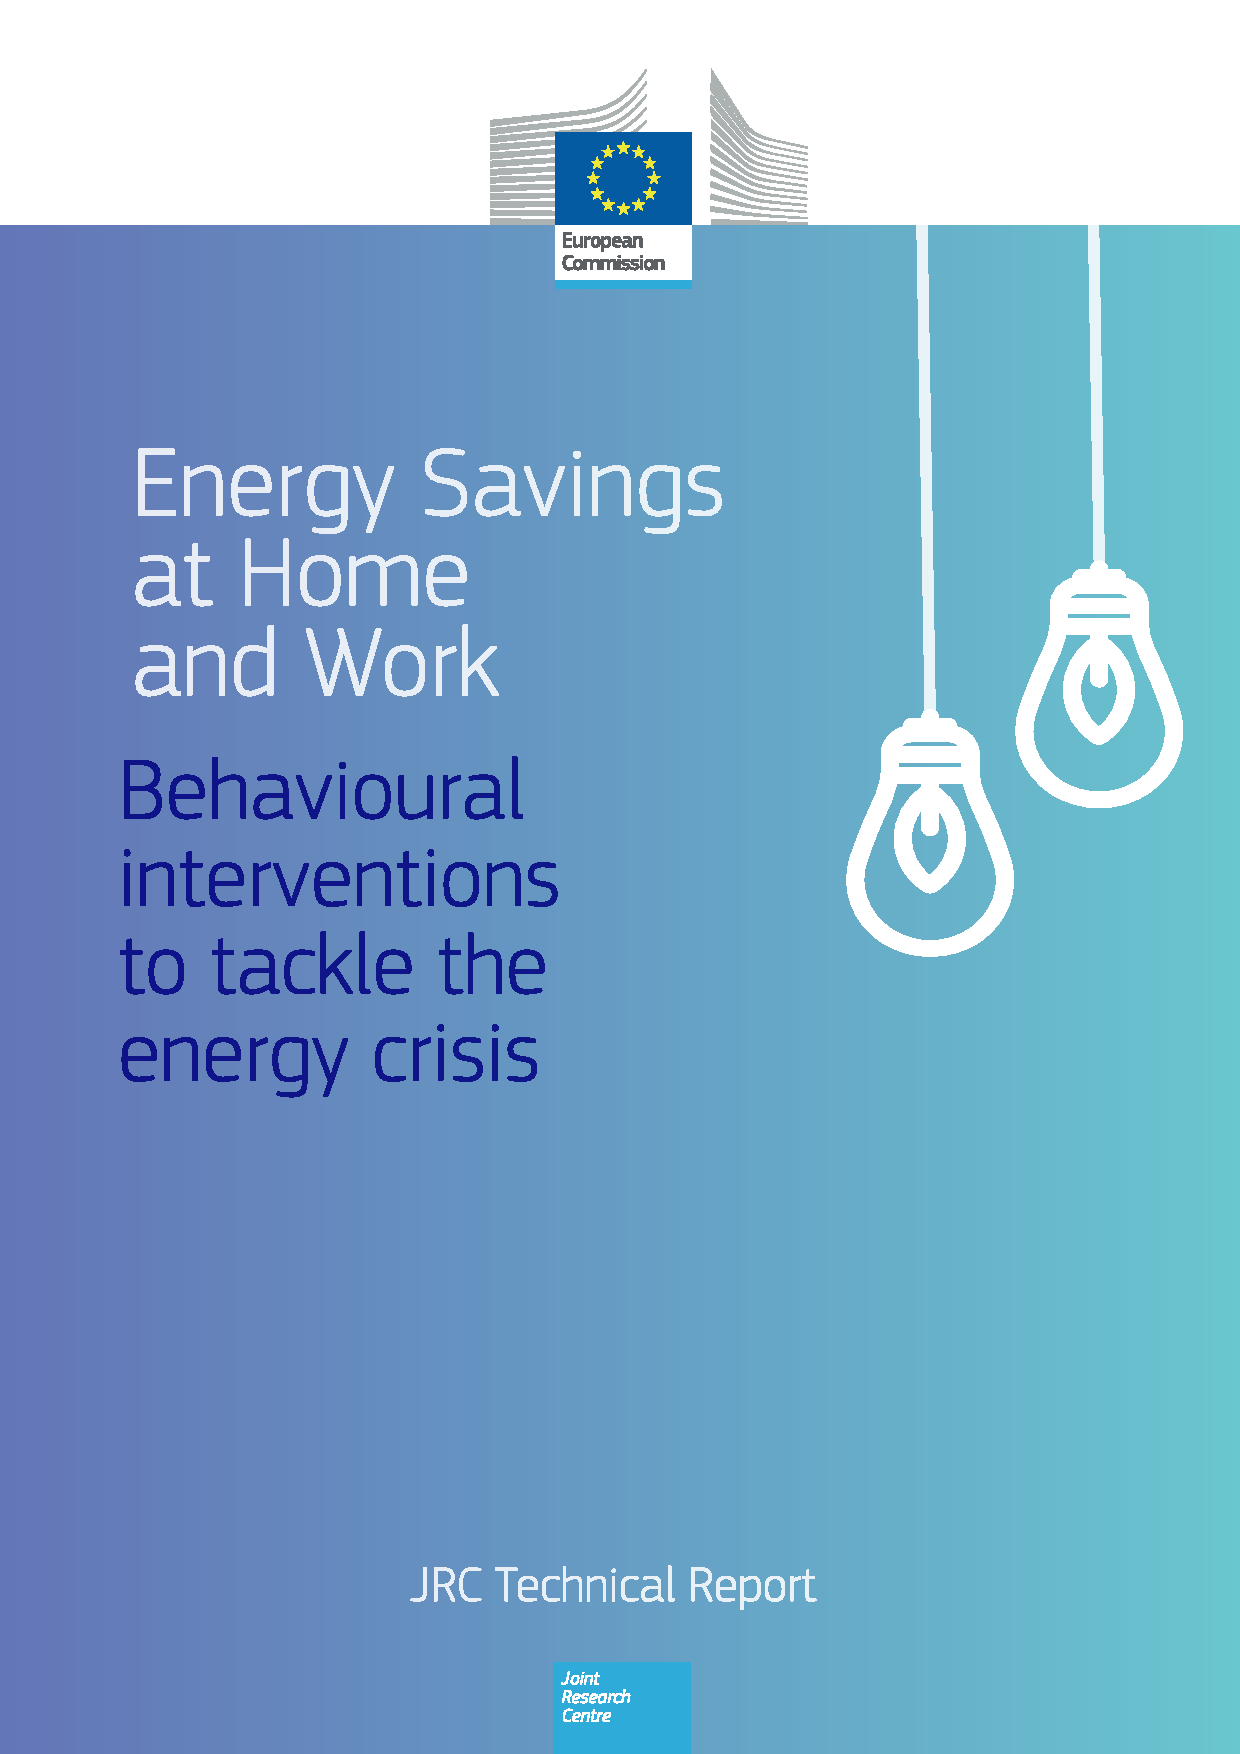
\includegraphics[width=\paperwidth,height=\paperheight,keepaspectratio]{cover_page.pdf}
  
    \vfill
\end{titlepage}
\restoregeometry

% Add title page
\newpage
\maketitle
\newpage

\begin{abstract}
Energy crises and concerns about climate change call for a decisive
shift in our daily behaviour at home and work. However, formulating
public policies encouraging and facilitating this change presents
considerable challenges. One key aspect is having an accurate
understanding of the behavioural factors influencing energy consumption
in residential and workplace settings and how people respond in
different contexts. This report reviews these behavioural factors,
discussing interventions to foster energy savings. It also spotlights
the conditions under which interventions targeting one context could
have an impact, `spillover', in another setting. The analysis highlights
the main similarities and differences between promoting energy savings
at home and work, such as differences in financial incentives,
awareness, cognitive barriers, free-riding problems, and peer
interactions. The report also provides recommendations for policies
incorporating spillovers, such as promoting habits, a green identity,
and peer influence.
\end{abstract}

\newpage 

% Notice page here


% Table of Contents
\renewcommand*\contentsname{Table of Contents}
\tableofcontents
\listoffigures
\listoftables
\clearpage 

% Line stretch 
\setstretch{1.15}

% Here is the main content ... 
\hypertarget{introduction}{%
\section{Introduction}\label{introduction}}

The path to climate neutral economy demands us to change habits. Since
changing habits is hard, governemnts must promote the change with
policies to foster energy savings and efficiency. These policies
typically involve individual-level and structural measures, such as X, Y
and Z. Events like Russia's invasion of Ukraine that create a sudden
shock in the energy supply, demand short-term policies. Designing these
policies can be challenging because (1) rising cost of energy (2)
curtailment is costly, especially for poor, (3) disruption of the
economy (4) economic uncertainty, etc. Behavioural interventions offer a
solution that is inexpensive and fast.

The halt on energy supply imports from Russia has multiple effects on
the path
\href{https://commission.europa.eu/strategy-and-policy/priorities-2019-2024/european-green-deal_en}{to
a climate-neutral European Union (EU)}. On the positive side, it forces
the EU to diversify its energy sources, accelerating the transition to
renewable energy and reducing fossil fuel dependence. However, there are
negative consequences, such as short-term energy shortages and increased
energy costs for households and businesses. The European Commission
proposed various measures to address the current situation outlined in
the
\href{https://commission.europa.eu/strategy-and-policy/priorities-2019-2024/european-green-deal/repowereu-affordable-secure-and-sustainable-energy-europe_en}{RePowerEU
plan}. The plan has two primary objectives: expediting investments in
diversifying the energy supply, mainly focusing on renewables, and
encouraging reductions in energy demand. The plan outlines
\emph{structural} and \emph{individual-level} measures to achieve these
objectives. Structural measures focus on achieving long-term effects,
such as creating new infrastructures, while individual-level measures
tend to have more immediate impacts.

Russia's invasion has triggered two objectives --- (a) and (b). The
European Commission has proposed that Member States adopt voluntary
reductions and suggested a series of interventions to achieve these
reductions. These interventions could be categorized into
individual-level, such as xxxx, and structural, such as xxxx. The
individual-level interventions were outlined in the Playing My Part
campaign by the European Commission in collaboration with the IEA.

Following this communication, all member States agreed to voluntarily
reduce their energy consumption by XX\% and implemented various policies
to achieve this goa. According to Bruegel, several ms used campaigns and
\ldots{}

This report examines individual-level measures from a behavioural
perspective, discussing the potential for energy savings and efficiency
improvements. By doing so, we aim to address the following questions:
What strategies can governments employ to incentivise individuals and
businesses to conserve energy without enforcing expensive restrictions
on energy usage? What first line of action can governments implement,
and what are the possible long-term effects?

Expert studies underscore the considerable impact of behavioural
interventions in addressing energy consumption and its associated
environmental impacts. According to the \href{www.iea.org}{International
Energy Agency (IEA)}, behavioural interventions that promote small
changes in daily activities among households and businesses have the
potential to immediately lower energy demand by 5\% at a relatively low
cost.

Another ehavioural interventions' effectiveness varies between office
spaces and residential buildings. While residential buildings account
for a larger share of final energy consumption (households for 28\% and
commercial/public services for 14\%,
\href{https://ec.europa.eu/eurostat/databrowser/view/NRG_BAL_S/default/table?lang=en}{Eurostat,
Simplified energy balances}), office spaces have a 41\% higher energy
consumption per square meter than private households
(\href{http://www.indicators.odyssee-mure.eu/}{Odyssee database}).
Therefore, office space interventions could be relatively more
effective. At the same time, research suggests that people tend to
internalise better the benefits of saving energy at home than at work.

Perusing numerous experimental studies on behavioural interventions
promoting energy conservation, we provide a roadmap identifying
effective strategies to address the peculiarities of energy consumption
at home and work. We also highlight the difficulties in designing
effective behavioural interventions and evaluating these measures'
effectiveness.

Our analysis highlights that even though there are differences in how
people conserve energy at home versus in the office, the behaviours in
one setting can influence and spill over into the other. For example, if
someone is diligent about turning off lights and unplugging electronics
at home, they may be more likely to do the same at work.

Similarly, if someone sees energy-saving behaviours being encouraged or
rewarded in the workplace, they may also be more likely to adopt them at
home. However, these spillover effects complicate policy evaluation and
are complex to integrate into policy design.

Concerning how to incorporate spillovers into policy, the report
discusses ideas such as promoting habits, green identity, and peer
influence. At the same time, it also calls for more empirical studies to
test the effectiveness of these interventions.

The report also examines how spillovers may complicate evaluating
policies' effectiveness. For example, a policy incentivising energy
savings at home may simultaneously encourage more energy waste at work,
with unclear net effects on energy consumption.

This report is as follows. First, it discusses the academic literature
and the available scientific evidence on the effectiveness of policy
interventions targeting households (Section \ref{sec:home}) and those
targeting behaviours at work (Section \ref{sec:work}). It then discusses
integrating actions targeting residential or workplace behaviours into
uniform policy interventions to better account for possible spillover
effects between the two spheres (Section \ref{sec:spillovers}).

\hypertarget{sec:home}{%
\section{Saving energy at home}\label{sec:home}}

\begin{keypoints}
\begin{itemize}[leftmargin=*,labelsep=5mm]
    \item Policy interventions can promote changing behaviour at home or encouraging investment in energy-efficient appliances and home renovations.
    \item Employee behaviour significantly impacts energy consumption in commercial buildings, with lower energy conservation at work than at home.
    \item Weak incentives and lack of direct control over energy consumption contribute to lower energy conservation at work.
    \item Personal rewards, organisational support, and addressing intrinsic motivations can be effective strategies for achieving energy savings at work.
    \item Further research is needed to understand the drivers of energy use in the workplace, but various interventions have been tested.
\end{itemize}
\end{keypoints}

\begin{figure}
\centering
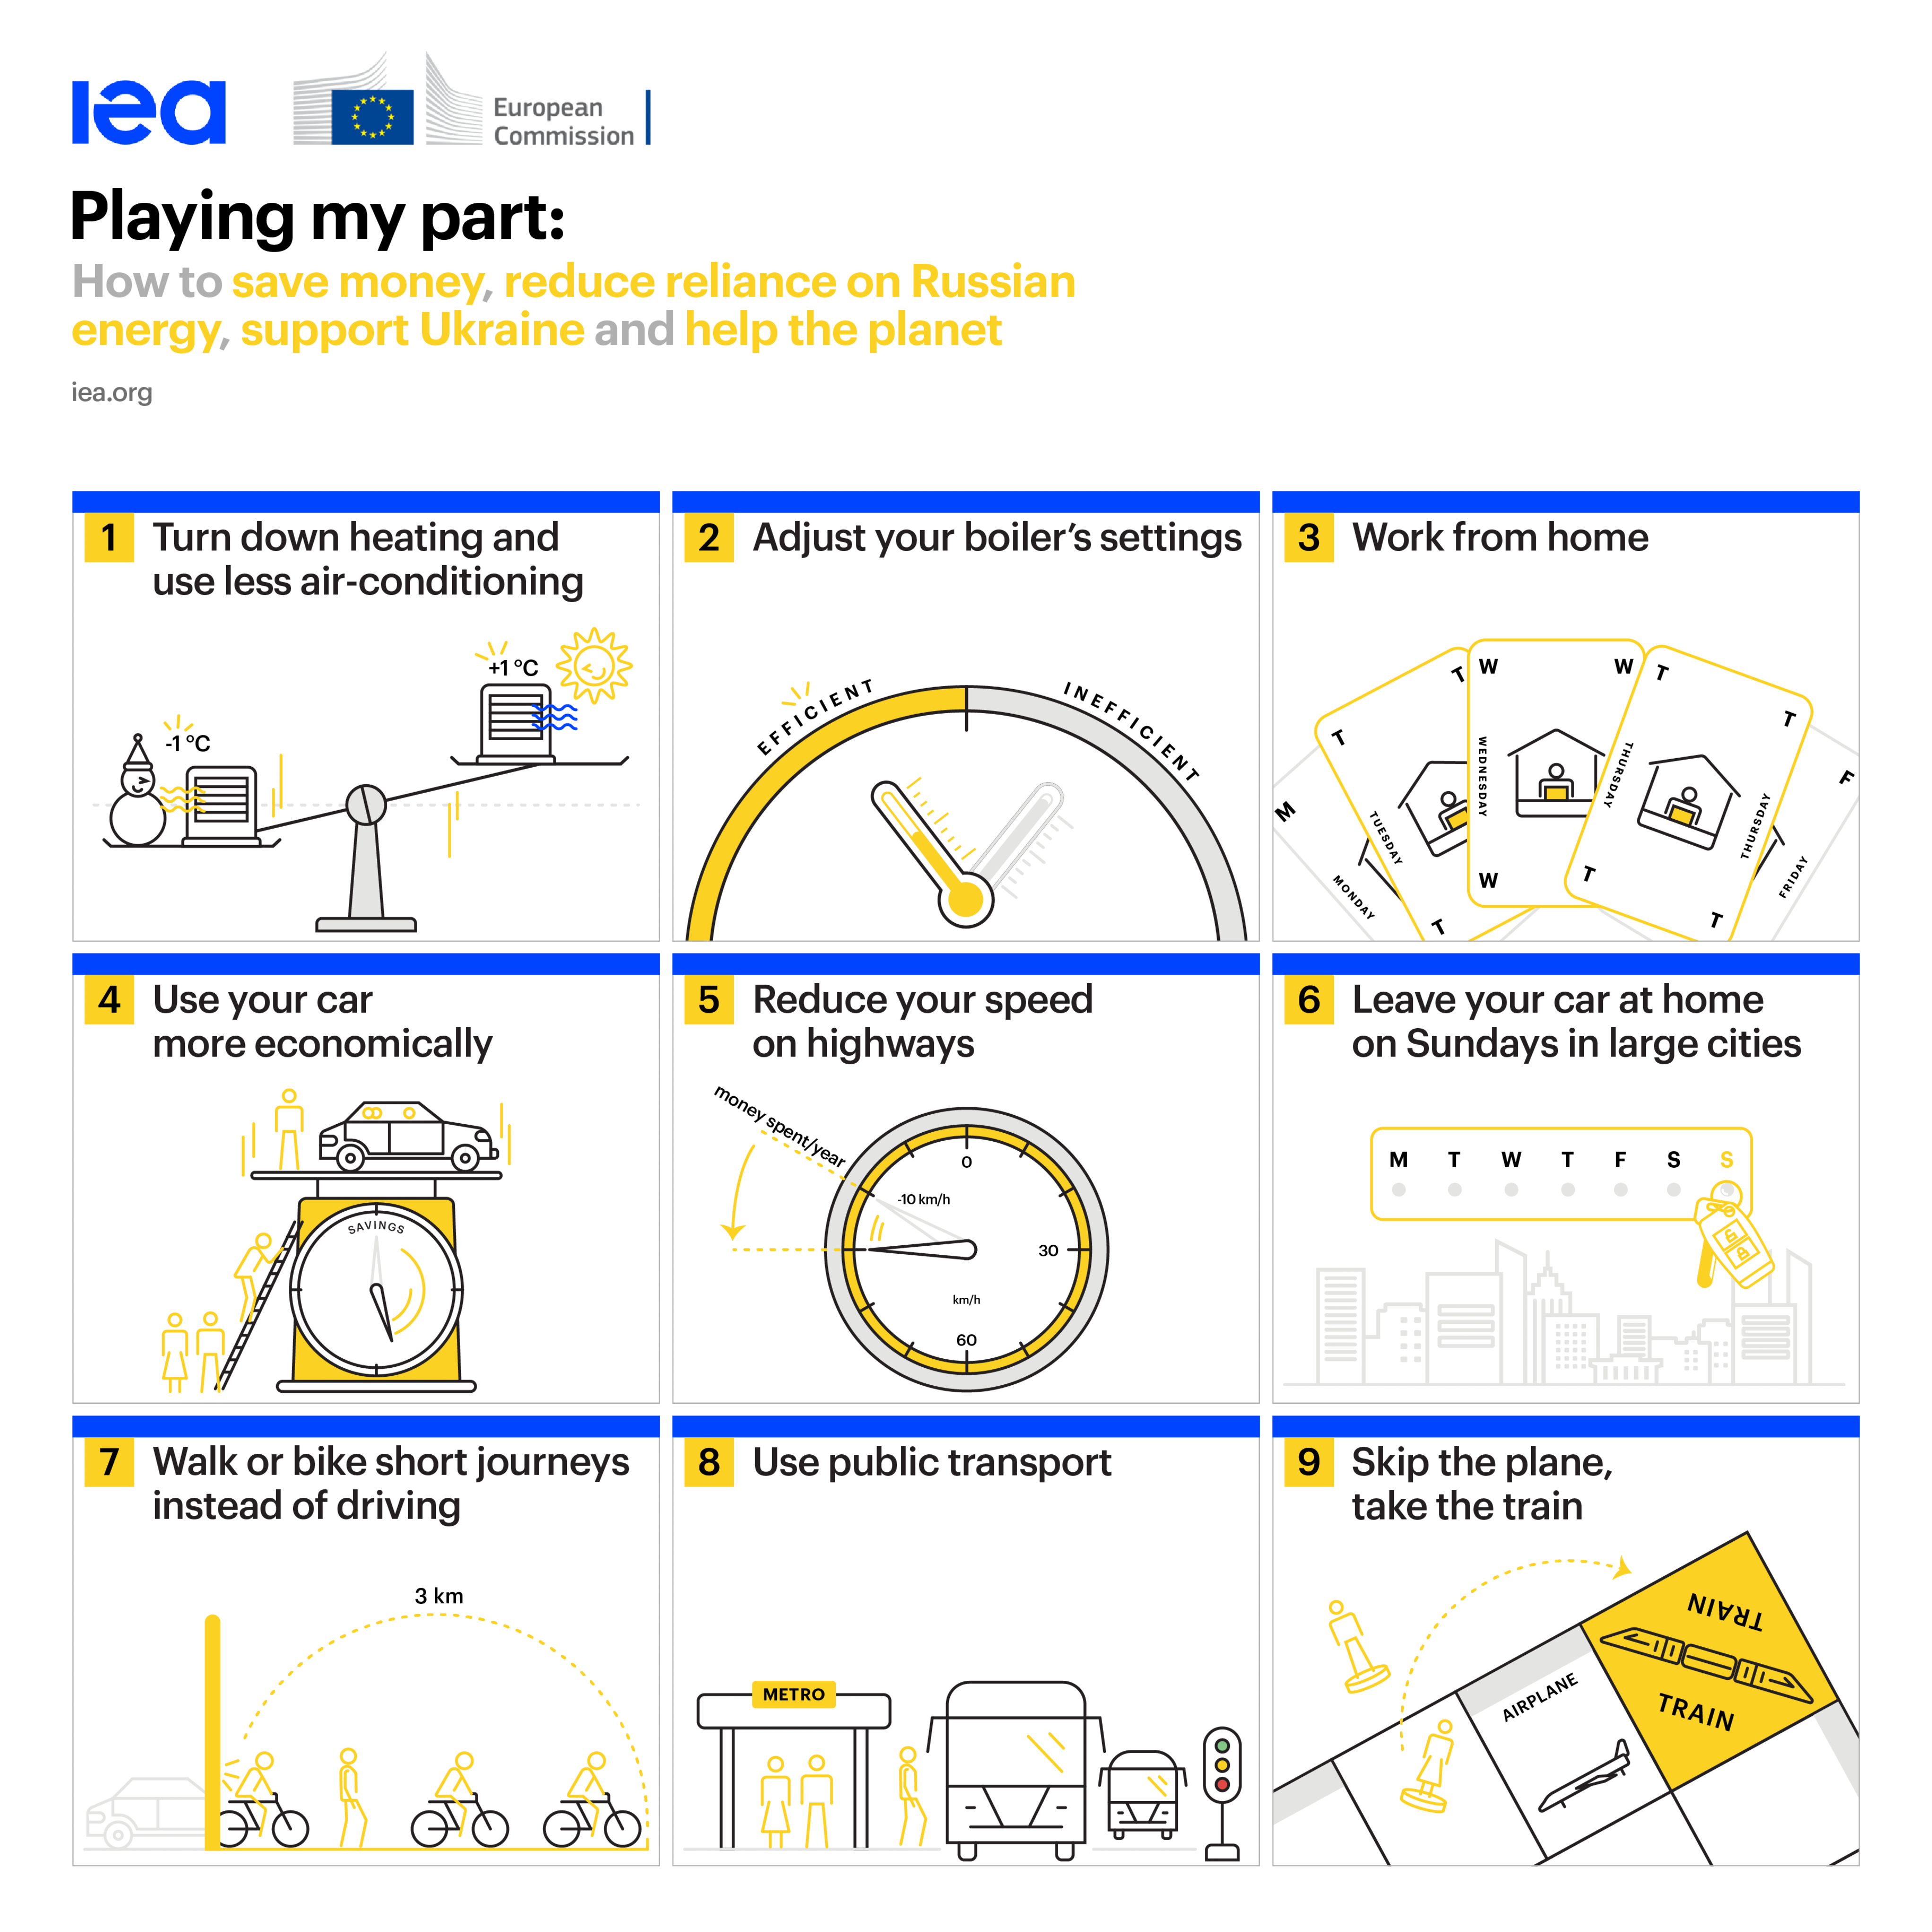
\includegraphics{Images/playingmypart-infographic.png}
\caption{Infographic from the ``Playing My Part'' information campaign
by the IEA and European Commission}
\end{figure}

Two different types of policy interventions promote energy savings among
households. The first approach involves encouraging families to change
their energy consumption behaviours, like turning off lights and
appliances when not used, cooking more efficiently, and reducing the use
of heating and cooling systems. Two different types of policy
interventions promote energy savings among households. The first
approach involves encouraging individuals to change their energy
consumption behaviours, like turning off lights and appliances when not
used, cooking more efficiently, and reducing the use of heating and
cooling systems.

The second approach involves stimulating purchases of energy-efficient
technologies, such as replacing traditional incandescent bulbs with new
LED ones, buying energy-efficient appliances, and installing ``smart''
home systems. Long-term strategies can also foster investments in home
renovations, from small renovations like replacing old windows to reduce
heat loss in the winter to installing photovoltaic panels.

In 2022, the European Commission combined both approaches in the
``Playing My Part'' information campaign, launched in response to the
rising energy costs for families after Russia invaded
Ukraine.\footnote{Information about the Playing My Part campaign is
  available at: \url{https://www.iea.org/reports/playing-my-part}
  {[}accessed December 21, 2022{]}.}

This campaign urged households, first and foremost, to adopt small
changes in their everyday energy consumption, such as adjusting their
boiler settings, turning down heating, using less air-conditioning, and
driving their cars more economically. Secondly, it also encouraged
households to switch to energy-efficient technologies, such as
purchasing electric heat pumps or installing programmable ``smart''
thermostats, while asking Member States to intensify the efforts to
facilitate the process.

However, it is difficult to anticipate how information campaigns like
``Playing My Part'' can influence people to reduce their energy
consumption during a crisis.

On the one hand, the recent increase in retail energy prices due to the
surge in wholesale prices caused by the embargo on Russia's fossil fuels
may cause people to be more concerned about the impact of higher energy
bills. Therefore, individuals may be more inclined to change their
energy usage and actively search for ways to reduce their energy
consumption to lower their bills. At the same time, government
interventions to calm energy prices, despite being necessary to offer
relief to individuals, could weaken the incentive for households to
achieve energy savings.

On the other hand, many studies have shown that, despite receiving basic
information about the potential benefits of good energy conservation
practices, only a minority of individuals tend to adopt such practices,
even when cost-effective (\protect\hyperlink{ref-jaffe1994energy}{Jaffe
and Stavins 1994}). This means that most individuals often stick to
their usual energy consumption patterns or habits rather than trying to
reduce their energy consumption.

\begin{keypoints}
Classical explanations for the Energy Paradox
\begin{itemize}

\item \textbf{Information barriers} Families face multiple barriers either in accessing information or absorbing it. For example, a study, based on a survey of Dutch households, shows that only about half of respondents are aware of their monthly charges for energy consumption, and only 40% understand the correct trade-off between different investment decisions in energy equipment [@brounen2013energy].

\item \textbf{Time discounting} Investments in energy efficiency and, to some extent, significant behavioural changes involve individual costs. These costs are typically immediate (i.e., installation expenses) offering only delayed rewards (i.e., lower electricty bills). However, if families heavily discount the future, they would rather spend their time or money elsewhere today.

\item \textbf{Heterogeneity in consumption}. Households are widely heterogeneous concerning their energy consumption patterns. Thus, even if a technology (or behaviour) is profitable on *average*, it may remain unattractive for a large portion of the population.

\end{itemize}
\end{keypoints}

The above explanations assume that individuals would make optimal
decisions if they had more information about costs and benefits or if
the market offered them more personalized solutions to save energy.
However, much psychology and behavioural economics evidence have
challenged these assumptions because people do not typically make
optimal decisions, if under the best conditions. On the contrary,
individuals often act as if they were predictably ``irrational'' or
biased.

Based on such evidence, other explanations for the Energy Paradox have
emerged. Here, we provide two examples:

\begin{itemize}
\item
  \textbf{Time-inconsistent preferences}. People often delay or postpone
  action despite knowing there will be negative consequences, a form of
  procrastination. This phenomenon is known as inconsistent time
  preferences, where people make choices today that are inconsistent
  with their future well-being and preferences. For example, people
  prefer to keep their heating systems at high levels to stay warm and
  comfortable, but they systematically regret their decision when they
  receive a high energy bill. For example, a recent study based on a
  survey with an experimental design shows that people who exhibited
  time-inconsistent preferences also tended to over-consume energy at
  home (\protect\hyperlink{ref-werthschulte2021role}{Werthschulte and
  Löschel 2021}).
\item
  \textbf{Loss aversion}. Another example is that, when making energy
  decisions, individuals may find it too costly to deviate from their
  current energy consumption patterns or ``status quo'' because it
  involves giving up their current comfortable lifestyle, which they
  have become accustomed to. Therefore, they may resist making changes,
  even if the potential rewards are significant, due to the fear of
  loss. This phenomenon is known as loss aversion, where people fear
  losses more than they seek equivalent gains. A recent study, based on
  a large-scale survey of EU citizens, shows that individuals who are
  loss averse are less likely to invest in energy-efficient appliances
  or retrofit measures
  (\protect\hyperlink{ref-schleich2019large}{Schleich et al. 2019}).
\end{itemize}

The reasons for the Energy Paradox remain a question still being
studied, and the behavioural factors influencing households' energy
decisions are still unclear. So, in this report, we take a more
practical approach by exploring different interventions found to be
successful in the academic literature. This will help us understand the
challenges and effectiveness of other solutions.

Table \ref{tab:households} summarises the interventions discussed below.

\hypertarget{information-nudges-and-energy-labels}{%
\subsection{Information nudges and energy
labels}\label{information-nudges-and-energy-labels}}

Information Nudges is a term used to describe policies sending
households energy-saving tips or rules of thumb to induce desired energy
consumption choices or rectify behavioural biases. These messages are
typically sent via electricity bills, postcards, emails, and other
media.

Extensive literature shows that Information Nudges are an effective way
to promote energy savings
(\protect\hyperlink{ref-craig1978assessing}{Craig and McCann 1978};
\protect\hyperlink{ref-ruokamo2022effect}{Ruokamo et al. 2022};
\protect\hyperlink{ref-dellavalle2020nudging}{DellaValle and Sareen
2020}; \protect\hyperlink{ref-caballero2021tackling}{Caballero and Della
Valle 2021}). However, multiple factors influence the effectiveness of
such measures, including the credibility of the source
(\protect\hyperlink{ref-craig1978assessing}{Craig and McCann 1978}), the
delivery method, and the target groups.

At the same time, the impact on energy consumption is of modest size. A
recent meta-analysis based on 52 studies between 2005 and 2020
(\protect\hyperlink{ref-buckley2020prices}{Buckley 2020}) shows that the
average effect of Information Nudges ranges between 2\% and 4\%. Despite
the modest effect size, they are typically inexpensive and easy to
deploy and the associated cost-effectiveness prompts their use.

Energy Labels are another form of information nudging as they serve to
intuitively convey a technology's or commodity's energy efficiency
properties. Extensive evidence has proven their effectiveness in various
settings, like energy-efficient electric appliances
(\protect\hyperlink{ref-dyer1988evaluation}{Dyer and Maronick 1988};
\protect\hyperlink{ref-dellavalle2019can}{DellaValle and Zubaryeva
2019}) and residential buildings
(\protect\hyperlink{ref-taranu2018closer}{Taranu and Verbeeck 2018};
\protect\hyperlink{ref-brounen2011economics}{Brounen and Kok 2011}) tend
to promote investments in long-term energy savings. One common
explanation for the efficacy of energy labels is that they provide
easy-to-grasp information and make the long-term impact of energy
expenses more salient, thus helping households to overcome
time-inconsistent decision patterns.

\hypertarget{energy-one-stop-shops}{%
\subsection{Energy one-stop shops}\label{energy-one-stop-shops}}

One-stop shops are agencies that aim to offer integrated solutions and
customer-centric services that simplify the decisional process for the
renovation of residential buildings. Indeed, increasing the efficiency
of residential buildings through renovations is challenging. It involves
a cumbersome and lengthy process in a fragmented market that might
discourage consumers. Interventions promoting one-stop shops can bridge
the fragmented demand and supply of the renovation value chain. These
shops guide citizens and businesses through the renovation journey, from
start to finish, and help them overcome hurdles they would otherwise
face alone. One-stop shops are relatively new, and so far, 63 case
studies have been identified and analysed in Europe
(\protect\hyperlink{ref-bertoldi2021role}{Bertoldi et al. 2021})
providing early evidence of their effectiveness.

\hypertarget{individual-feedback-and-goal-setting}{%
\subsection{Individual feedback and goal
setting}\label{individual-feedback-and-goal-setting}}

Personalised feedback promotes energy savings by informing households of
their energy consumption. There is widespread evidence of their
effectiveness, as outlined in several comprehensive reviews
(\protect\hyperlink{ref-abrahamse2005review}{Abrahamse et al. 2005};
\protect\hyperlink{ref-andor2018behavioral}{Andor and Fels 2018}).
Personalised feedback aims to make energy consumption more ``visible''
to consumers. Electric companies typically send feedback via periodic
email or monthly electricity bills. Sometimes, consumers can receive
real-time feedback to adjust their energy consumption to price changes
during the day or avoid peaks using smart meters
(\protect\hyperlink{ref-aydin2018information}{Aydin, Brounen, and Kok
2018}). However, as technology progresses and new ways of communication
emerge, more work is needed on designing individual feedback to optimise
effectiveness in a fast-changing environment.

Setting specific household energy consumption goals is another critical
application of individual feedback. A recent meta-analysis of studies
that combine feedback with goal settings shows that this combination
consistently reduces the energy consumption of private households
(\protect\hyperlink{ref-andor2018behavioral}{Andor and Fels 2018}). Yet,
the effect sizes can vary considerably, suggesting that contextual
factors influence the success of policy implementation.

\hypertarget{intrinsic-motivations-and-social-norms}{%
\subsection{Intrinsic motivations and social
norms}\label{intrinsic-motivations-and-social-norms}}

In addition to providing information in an easily understandable manner
to consumers, behavioural interventions can impact energy savings by
targeting individuals' inner (intrinsic) motivation to save energy. For
example, interventions can appeal to individuals' environmental values
or willingness to adhere to well-established social norms. These
interventions assume that people are intrinsically motivated to save
energy and will respond to solicitations without personal benefits or
financial incentives (\protect\hyperlink{ref-van2015social}{Van der
Linden 2015}).

One specific example of behavioural interventions that use the power of
social norms consists of providing individuals with information about
how much energy is used by peers or socially approved energy consumption
levels, thus supplying social comparisons and norms. Since many
individuals care about conforming, this information motivates them to
change their energy consumption. Extensive literature has shown the
effectiveness of this approach in promoting energy savings
(\protect\hyperlink{ref-allcott2011social}{Allcott 2011};
\protect\hyperlink{ref-caballero2021tackling}{Caballero and Della Valle
2021}).

\hypertarget{warnings-and-fact-checking}{%
\subsection{Warnings and
fact-checking}\label{warnings-and-fact-checking}}

Misinformation is an obstacle to energy savings and environmentally
conscious behaviours, like other informational barriers. For example,
studies have shown widespread energy misinformation about politicised
topics such as the causes of global climate change
(\protect\hyperlink{ref-oreskes2004scientific}{Oreskes 2004};
\protect\hyperlink{ref-farrell2019evidence}{Farrell, McConnell, and
Brulle 2019}), and fake news underplaying the concerns about climate
change can negatively influence people's perception of the problem and
their willingness to invest in energy-efficient technology. Similarly,
misinformation about energy use could also affect long-term policies of
supply diversification, for example, by giving citizens a wrong idea of
the risks of nuclear power (\protect\hyperlink{ref-ho2018can}{Ho et al.
2018}, \protect\hyperlink{ref-ho2022fake}{2022};
\protect\hyperlink{ref-ho2019environmental}{Ho and Kristiansen 2019}).

Behavioural interventions, such as warnings and fact-checking, offer a
promising approach to ``inoculate'' public attitudes against the spread
of misinformation about energy policies. For example, a recent
experimental survey shows that warning people about politically
motivated attempts to spread misinformation is an effective way to fight
the spread of misinformation on climate change
(\protect\hyperlink{ref-van2015social}{Van der Linden 2015}). However,
more work is needed to understand what works against misinformation.

\begin{longtable}[]{@{}
  >{\raggedright\arraybackslash}p{(\columnwidth - 2\tabcolsep) * \real{0.2973}}
  >{\raggedright\arraybackslash}p{(\columnwidth - 2\tabcolsep) * \real{0.6757}}@{}}
\caption{Intereventions promoting energy conservation at home
\label{tab:households}}\tabularnewline
\toprule()
\begin{minipage}[b]{\linewidth}\raggedright
\textbf{Intervention}
\end{minipage} & \begin{minipage}[b]{\linewidth}\raggedright
\textbf{Definition}
\end{minipage} \\
\midrule()
\endfirsthead
\toprule()
\begin{minipage}[b]{\linewidth}\raggedright
\textbf{Intervention}
\end{minipage} & \begin{minipage}[b]{\linewidth}\raggedright
\textbf{Definition}
\end{minipage} \\
\midrule()
\endhead
\textbf{~} & ~ \\
\textbf{Information nudges} & Energy-saving tips or energy-efficiency
information through energy labels. \\
\textbf{~} & ~ \\
\textbf{One-stop shops} & Agencies to guide citizens and businesses
through the entire process of energy renovation. \\
\textbf{~} & ~ \\
\textbf{Feedback \& goals} & Personalized information about energy
consumption to make it more visible to consumers. Personalized feedbacks
can be also used for goal setting. \\
\textbf{~} & ~ \\
\textbf{Social comparisons} & Providing information about energy
consumption by peers to activate social norms of energy conservation. \\
\textbf{~} & ~ \\
\textbf{Warnings \& fact-checking} & Warning people against
misinformation about climate change, the risks of nuclear power, etc. \\
\bottomrule()
\end{longtable}

\hypertarget{takeaways}{%
\subsubsection*{Takeaways}\label{takeaways}}
\addcontentsline{toc}{subsubsection}{Takeaways}

\begin{itemize}
\item
  Encouraging energy savings is difficult due to households' information
  barriers, misinformation, heavily discounted future efficiency gains,
  heterogeneity, and cognitive barriers in energy consumption
  decision-making.
\item
  Several behavioural interventions address these problems adequately.

  \begin{itemize}
  \item
    \textbf{Information barriers:} information nudges, energy labels,
    warnings, fact-checking
  \item
    \textbf{Cognitive and effortful process:} information nudges, energy
    labels, one-stop energy shops
  \item
    \textbf{Motivation:} feedback, goal setting, social norm
    interventions
  \end{itemize}
\end{itemize}

\hypertarget{sec:work}{%
\section{Saving energy at work}\label{sec:work}}

\begin{keypoints}
\begin{itemize}[leftmargin=*,labelsep=5mm]
    \item Policy interventions can focus on changing employee behaviour or encouraging management to invest in energy-efficient technologies.
    \item Employee behaviour significantly impacts energy consumption in commercial buildings, with lower energy conservation at work than at home.
    \item Weak incentives and lack of direct control over energy consumption contribute to lower energy conservation at work.
    \item Personal rewards, organisational support, and addressing intrinsic motivations can be effective strategies for achieving energy savings at work.
    \item Further research is needed to understand the drivers of energy use in the workplace, but various interventions have been tested.
\end{itemize}
\end{keypoints}

The focus on interventions stimulating behavioural change at work is
partly motivated by evidence showing that employee behaviour
significantly impacts the energy consumption of commercial buildings
(\protect\hyperlink{ref-azar2014comprehensive}{Azar and Menassa 2014}).
At the same time, other evidence shows that, while at work, people make
fewer energy conservation actions than at home
(\protect\hyperlink{ref-lin2019mixing}{Lin and Azar 2019}).

One reason for fewer energy conservation actions at work is that
employees typically have weak incentives to save energy in the
workplace. People are better off in warm rather than cold offices, using
air-conditioning in the summer; and they may feel less of a personal
connection with energy wastes, such as forgetting to turn off the office
lights or computer when leaving, than at home.

Another reason is that employees may feel they have no direct control
over the energy systems, which are usually centralised. Such centralised
systems have two mean implications for energy consumption. On the one
hand, centralised systems may help facility managers oversee the
buildings and generate energy savings. On the other, these systems could
prevent energy conservation actions by the occupants, such as turning
off the lights when not needed.

One possible solution is to offer rewards when staff achieves specific
energy-saving goals at the individual or organisational level. For
example, transportation companies often reward their drivers with cash
bonuses or vouchers for consuming less fuel than predetermined levels
(\protect\hyperlink{ref-schall2017incentivizing}{Schall and Mohnen
2017}). However, such compensation schemes can clash with productivity
goals when, for example, organisations cannot track individual energy
consumption for technical or privacy reasons, and employees have the
incentive to free-ride on each other.

Other solutions could involve adequate organisational support or
creating new opportunities for energy conservation actions. Research
based on surveys suggests that employees view the lack of financial
incentives for energy savings as less of a factor than missing
organisational support, limited opportunities for energy conservation,
little time, or even confusion about who has the assigned responsibility
to initiate energy savings
(\protect\hyperlink{ref-li2019understanding}{Li et al. 2019};
\protect\hyperlink{ref-staddon2016intervening}{Staddon et al. 2016}).

Additionally, intrinsic motivations, such as environmental concerns or
for the organisation's mission and image, and warm-glow feelings can
partially compensate for the lack of incentives or organisational
support. Several studies have shown that people are willing to
contribute to the workplace environment because of their intrinsic
motivations, which are fundamental to leading employees to save energy
in the workplace (\protect\hyperlink{ref-leygue2017saving}{Leygue,
Ferguson, and Spence 2017}).

However, the drivers of energy use in the workplace still need to be
better understood. Large-scale empirical studies considering the vast
heterogeneity of organisations and behaviours are missing. Despite this
limitation, several policy interventions have been tested to change
energy-use behaviour in the workplace
(\protect\hyperlink{ref-staddon2016intervening}{Staddon et al. 2016}).
These interventions can be broadly grouped into three main categories,
as in Table \ref{tab:firms}. Below, we discuss a few examples.

\hypertarget{information-social-norms-and-peer-education}{%
\subsection{Information, Social Norms, and Peer
Education}\label{information-social-norms-and-peer-education}}

\hypertarget{information-social-norms-peer-education}{%
\subsection{Information, social norms, \& peer
education}\label{information-social-norms-peer-education}}

Field experiments evaluated the effectiveness of comparative feedback.
For example, Carrico and Reimer
(\protect\hyperlink{ref-carrico2011motivating}{2011}) show that
comparative feedback on energy consumption (based on different office
buildings) achieved 7\% and 4\% energy savings, respectively, compared
to an \emph{increase} in energy consumption associated with sending
informative postcards. Remarkably, such comparative feedback appears
effective in widely different settings, even in the industrial sector, a
metallurgical company as in Siero et al.
(\protect\hyperlink{ref-siero1996changing}{1996}), and there is evidence
of long-term effects after removing the comparative feedback
(\protect\hyperlink{ref-kamilaris2015case}{Kamilaris et al. 2015}).

Comparative feedback in the workplace can also help coordination and
decision-making, such as when using air-conditioning and ventilation in
shared spaces or when energy consumption requires some form of consensus
among employees. For example, in one notable field experiment
(\protect\hyperlink{ref-murakami2007field}{Murakami et al. 2007}),
employees could submit their preferences on air conditioning use in
real-time with an algorithm providing individual feedback on air
conditioning preferences coupled with energy-saving information. The
results showed that the algorithm recommendations promoted coordination
and produced significant energy savings.

\hypertarget{monetary-and-non-monetary-rewards}{%
\subsection{Monetary and non-monetary
rewards}\label{monetary-and-non-monetary-rewards}}

Several studies have shown that non-monetary rewards, including
vouchers, public social reward points
(\protect\hyperlink{ref-handgraaf2013public}{Handgraaf, De Jeude, and
Appelt 2013}), serious games
(\protect\hyperlink{ref-orland2014saving}{Orland et al. 2014}) or the
possibility of winning a competition, can reduce energy consumption. For
example, a study testing the promotion of energy saving based on points
engaged about 60\% of employees, leading to a substantial reduction in
energy consumption (\protect\hyperlink{ref-kuntz2012many}{Kuntz, Shukla,
and Bensch 2012}).

In a serious game called ``Energy Chickens'', energy saving measured
through plug-in sensors earned participants eggs with which they could
purchase accessories in a virtual farm. The intervention led to
significant energy savings; however, the effects did not seem to last
beyond duration of the game
(\protect\hyperlink{ref-orland2014saving}{Orland et al. 2014}).
Similarly, a large-scale competition involving small material rewards
among 500 Italian bank branches also reduced energy consumption
(\protect\hyperlink{ref-fanghella2022evaluating}{Fanghella, D'Adda, and
Tavoni 2022}).

\hypertarget{default-settings-and-automation}{%
\subsection{Default Settings and
Automation}\label{default-settings-and-automation}}

Introducing defaults and automation can significantly impact energy
saving (\protect\hyperlink{ref-staddon2016intervening}{Staddon et al.
2016}). Advanced power strips which automatically switch off computer
screens or non-essential circuits can save up to 20\% of energy
consumption (\protect\hyperlink{ref-sheppy2014reducing}{Sheppy et al.
2014}). Also, automatically reducing heating at the end of a workday or
before weekends is a promising technological solution to energy
over-consumption. However, setting the correct temperature or reasonable
defaults is challenging. In one field experiment, researchers found that
lowering the default room temperature by 1 or 2 degrees in offices could
increase energy consumption as the occupants are more likely to overrule
the defaults (\protect\hyperlink{ref-brown2013testing}{Brown et al.
2013}).

Another issue is how defaults could create a differential impact among
employees. In response to the current energy crisis caused by Russia's
invasion of Ukraine, many local and national governments defaulted 19
degrees in public buildings to save gas consumption. However, while
studies on the effectiveness of this default are rare, anecdotal
evidence suggests that this decision may negatively affect workers with
special needs and ignores individual perceptions of temperature and
comfort.

\textbf{Takeaways}

\begin{itemize}
\item
  Policy interventions for energy savings at work can focus on behaviour
  change or investment in energy-efficient technologies.
\item
  Lack of direct financial incentives, organisational support, and
  limited energy conservation opportunities influence employee energy
  consumption. Intrinsic motivations can partially compensate for the
  lack of incentives or support.
\item
  Evidence points to effective behavioural interventions addressing
  these problems.

  \begin{itemize}
  \item
    \textbf{Information \& Feedback}: comparative feedback activates
    social norms and effectively encourages energy savings.
  \item
    \textbf{Internal competitions \& non-monetary rewards:} prizes
    promote energy savings and activate image and reputation concerns
    that will likely enhance social norm interventions.
  \item
    \textbf{Defaults \& automation:} Defaults can considerably impact
    energy consumption, but setting the appropriate default is
    challenging and should consider various behavioural responses,
    including the risk of disparities.
  \end{itemize}
\end{itemize}

\begin{longtable}[]{@{}
  >{\raggedright\arraybackslash}p{(\columnwidth - 2\tabcolsep) * \real{0.3194}}
  >{\raggedright\arraybackslash}p{(\columnwidth - 2\tabcolsep) * \real{0.6806}}@{}}
\caption{Intereventions promoting energy conservation at work
\label{tab:firms}}\tabularnewline
\toprule()
\begin{minipage}[b]{\linewidth}\raggedright
\textbf{Intervention}
\end{minipage} & \begin{minipage}[b]{\linewidth}\raggedright
\textbf{Definition}
\end{minipage} \\
\midrule()
\endfirsthead
\toprule()
\begin{minipage}[b]{\linewidth}\raggedright
\textbf{Intervention}
\end{minipage} & \begin{minipage}[b]{\linewidth}\raggedright
\textbf{Definition}
\end{minipage} \\
\midrule()
\endhead
\textbf{~} & ~ \\
\textbf{Feedback} & Targeted feedback (hints, suggestions, performance,
etc.) to enable individuals to reflect and adapt their behaviour. \\
\textbf{~} & ~ \\
\textbf{Explicit incentives} & Increase motivation by awarding people
monetary or non-monetary rewards \\
\textbf{~} & ~ \\
\textbf{Defaults \& automation} & Exploits the tendency of people to
generally accept the default option in a specific situation. \\
\bottomrule()
\end{longtable}

\hypertarget{sec:spillovers}{%
\section{Spillovers and Peer Effects}\label{sec:spillovers}}

\begin{tcolorbox}[colback=yellow!10,colframe=black]
\textbf{Key Points: Spillovers and Peer Effects}
\begin{itemize}[leftmargin=*,labelsep=5mm]
    \item Energy conservation policies at home and work are interconnected through spillovers, which refer to the effects of policy interventions on non-targeted behaviours.
    \item Spillovers can be positive or negative, impacting the overall effectiveness of a policy.
    \item Types of spillovers include behavioural, temporal, contextual, and social spillovers, each with its own characteristics and implications.
    \item Evidence shows the existence of spillovers in energy conservation, such as rebound effects, temporal spillovers in retrofitting behavior, contextual spillovers in food waste reduction, and social spillovers in the adoption of clean energy technologies.
    \item Understanding and leveraging spillovers can enhance policy design and evaluation, with strategies like promoting habit formation, fostering a green identity, encouraging commitment, addressing moral licensing, and leveraging peer effects.
\end{itemize}
\end{tcolorbox}

Even though we have treated policies promoting energy conservation at
home and work separately so far, they are strongly interlinked. The
concept of ``spillover'' is often used to describe this connection, as
it refers to the effects of policy interventions on multiple
non-targeted behaviours.

Spillovers can be positive or negative depending on whether the effects
on the non-targeted behaviours are in the direction of the desired
change. This distinction is essential to understand the net effect of a
policy. For example, a policy that positively affects the targeted
behaviour may still produce a net negative result if the adverse effects
on off-target behaviours offset the positive ones.

One critical step in the analysis of spillovers is to identify areas or
situations where they may arise. A deep analysis of the academic
literature by Nilsson and others
(\protect\hyperlink{ref-nilsson2017spillover}{2017}) suggests
classifying spillovers into various types based on the following
distinctions (see also Table \ref{tab:spillovers}):

\begin{itemize}
\item
  \textbf{Behavioural Spillovers.} This category refers to the effects
  of one behavioural intervention on non-targeted behaviours. For
  example, a policy reducing households' electricity consumption by
  raising individuals' environmental concerns could also affect people's
  inclinations towards recycling, eco-driving, and other non-targeted
  pro-environmental behaviours.
\item
  \textbf{Temporal Spillovers.} These spillovers occur when the effect
  of one behavioural intervention at a given time also influences the
  same behaviour in the future. For example, educating children to save
  energy will affect their current behaviour, but it could also
  influence their behaviour later in life.
\item
  \textbf{Contextual Spillovers}. These arise when the effect of one
  behavioural intervention transfers from one context to another. For
  example, interventions that persuade households to consume less energy
  at home could also stimulate energy savings at work.
\item
  \textbf{Social Spillovers}. These refer to the influence that choices
  by others may have on individual choices. Unlike other spillovers,
  they occur between individuals. For example, an intervention informing
  school children about energy savings at school could also affect the
  information, and thus energy consumption, of their family and friends.
\end{itemize}

Multiple studies have investigated spillovers in the context of energy
conservation. One such study is a meta-analysis of 22 experimental
studies, which provides evidence of significant behavioural spillovers
(\protect\hyperlink{ref-maki2019meta}{Maki et al. 2019}). One example of
spillover observed is the ``rebound effect,'' which refers to an
increase in consumption after an investment in energy-efficient
equipment. This may happen when the initial energy savings of the
equipment may lead to increased consumption, which can ultimately negate
the energy savings achieved through the investment
(\protect\hyperlink{ref-aydin2017energy}{Aydin, Kok, and Brounen 2017}).

A study by Egner and Klöckner
(\protect\hyperlink{ref-egner2021temporal}{2021}), based on a
large-scale survey of Norwegian households, found evidence of temporal
spillovers in energy retrofitting behaviour. Specifically, they found
that households who completed energy retrofits once were more likely to
retrofit their homes again three years later. These findings suggest
that the initial retrofitting behaviour had a positive spillover effect,
leading to continued interest and commitment to energy efficiency over
time.

Yet, there is still a need for more evidence on contextual spillovers in
energy consumption across home and work. However, in the context of food
waste, there is evidence of positive spillovers across these contexts. A
quasi-experimental study shows that efforts to reduce food waste in the
workplace are associated with food-saving actions at home
(\protect\hyperlink{ref-wang2021take}{Wang et al. 2021}).

In the context of energy conservation, there is evidence of a strong
positive association between energy consumption at home and work via
surveys (\protect\hyperlink{ref-littleford2014context}{Littleford,
Ryley, and Firth 2014}; \protect\hyperlink{ref-lin2019mixing}{Lin and
Azar 2019}). This association has been further tested in laboratory
experiments, which have confirmed a positive link
(\protect\hyperlink{ref-alt2022incentives}{Alt and Gallier 2022}).
However, there is still a need for more experimental evidence in the
field to better understand the potential for spillovers in energy
conservation across different contexts.

The evidence of social spillovers is also conspicuous. Research has
shown that solar cell deployment becomes more likely if the neighbours
have installed this technology on their roofs
(\protect\hyperlink{ref-bale2013harnessing}{Bale et al. 2013}). This
suggests that one individual or household's actions can influence
others' behaviour in their social network or neighbourhood, leading to a
ripple effect of energy conservation behaviour. By leveraging the power
of social spillovers and designing strategies that promote visible and
conspicuous displays of energy-saving behaviours, it may be possible to
increase the adoption of clean energy technologies and promote
sustainable behaviours more broadly.

The presence of spillovers in energy conservation has multiple
implications for policy design and evaluation. On the one hand, it
complicates the ex-ante cost-benefit analysis and ex-post impact
assessment of energy-conservation policies, as discussed by Galizzi and
others (\protect\hyperlink{ref-galizzi2019measure}{2019}). If a policy
intervention generates spillovers, ignoring these spillovers puts
policymakers at risk of underestimating or overestimating the actual
impact of one intervention. At the same time, estimating possible
spillovers in ex-ante and ex-post evaluations is generally complicated,
and more research is needed to provide an easy-to-use framework for
policy evaluation.

Regarding policy design, more research is needed to understand how
policymakers can leverage spillovers to enhance energy-saving
interventions. While the discussion continues, we examine key levers
widely studied in the literature as discussed below.

\hypertarget{habit-formation}{%
\subsection{Habit formation}\label{habit-formation}}

Social psychologists define a habit as a settled routine or regular
tendency triggered by exposure to the same environmental cues, for
example, turning off the lights when no one is using them. It follows
that once an energy-saving behaviour becomes an established habit, it
does not need nor require specific incentives or motivations to be
triggered, which makes habit formation a particularly appealing
objective for policies, as discussed elsewhere
(\protect\hyperlink{ref-van2019drivers}{Broek, Walker, and Klöckner
2019}).

Various studies examined interventions encouraging efficient
energy-consumption habits showing evidence that policies that stimulate
habit formation are effective. For example, Ito et al.
(\protect\hyperlink{ref-ito2018moral}{2018})~randomly assigned
households to a dynamic pricing scheme encouraging good energy
conservation habits. Results show that this approach produced
significant energy savings, most of which were thorough habit formation
as the treatment effect persisted even after the intervention had
ceased. This study underscores a more general idea suggesting that habit
formation could explain why one-shot behavioural interventions generate
results on energy conservation that continue over time
(\protect\hyperlink{ref-allcott2014short}{Allcott and Rogers 2014};
\protect\hyperlink{ref-jessoe2014knowledge}{Jessoe and Rapson 2014}).

\hypertarget{identity}{%
\subsection{Identity}\label{identity}}

One way to leverage contextual spillovers is through interventions
encouraging people to adopt a green identity. If people consider
themselves environmentalists, as this notion is part of their identity,
they will show consistent pro-environmental behaviours in multiple
contexts.

Although the evidence on these spillovers is limited, a survey of the UK
public shows that people who self-identify as environmentalists tend to
maintain pro-environmental behaviour in multiple contexts
(\protect\hyperlink{ref-whitmarsh2010green}{Whitmarsh and O'Neill
2010}). Moreover, some studies have tested different interventions to
foster individuals' environmental identity. These studies have shown
that using cues from past pro-environmental behaviour and feedback to
label a person as an environmentalist can effectively stimulate a
pro-environmental identity
(\protect\hyperlink{ref-geng2019globalize}{Geng, Sarkis, and Bleischwitz
2019}; \protect\hyperlink{ref-gleue2022identity}{Gleue et al. 2022};
\protect\hyperlink{ref-fanghella2019use}{Fanghella, d'Adda, and Tavoni
2019}).

\hypertarget{commitment-to-the-cause}{%
\subsection{Commitment to the cause}\label{commitment-to-the-cause}}

Committing to engage pro-environmentally can positively affect
spillovers. Such a commitment can occur in the form of pledges but also
in the form of actual behaviour. Inclining in costly or effortful
behaviour for the environment's sake can be considered a self-signal of
being committed to a pro-environmental goal. As a consequence,
subsequent pro-environmental actions in other contexts become more
likely. Through these self-signals, commitments are highly linked to the
establishment of an environmental identity to which the respective
actions positively contribute.

There exists evidence that people who gave up on their monetary income
for a good cause have been less likely to seize benefits at the expense
of others when having the opportunity to thereafter
(\protect\hyperlink{ref-gneezy2012paying}{\textbf{gneezy2012paying?}}).
This shows that commitments in pledges and actions can act as a ``foot
in the door'', helping people to focus on a specific goal or objective.

\hypertarget{moral-licensing}{%
\subsection{Moral licensing}\label{moral-licensing}}

Contextual spillovers can also be harmful to energy conservation. For
example, a policy that targets household energy savings may succeed in
reducing energy consumption at home but inadvertently increase energy
consumption at work, with an overall effect that could vary from
positive to negative.

One frequent explanation for negative spillovers implicates the concept
of ``moral licensing,'' which describes a situation in which past good
deeds will lower the probability of engaging in future good behaviours
(\protect\hyperlink{ref-merritt2010moral}{Merritt, Effron, and Monin
2010}). Moral licensing is part of a more general theory of moral
balancing (\protect\hyperlink{ref-funder1991explorations}{Funder and
Colvin 1991}; \protect\hyperlink{ref-monin2001moral}{Monin and Miller
2001}), which describes how past actions could affect the probability of
engaging in future behaviours, either good/moral or wrong/immoral.

Several studies have examined moral licensing in various settings to
assess the magnitude of these effects. For instance, a meta-analysis of
91 state-of-the-art experiments shows the effect size of moral licensing
can be considerable (\protect\hyperlink{ref-blanken2015meta}{Blanken,
Van De Ven, and Zeelenberg 2015}). However, we need more studies focused
on the effects of moral licensing on energy consumption.

How moral licensing relates to policies is still a largely unexplored
topic. However, using an experiment in the context of charitable
donations, a recent study shows that interventions offering monetary
incentives to adopt pro-environmental behaviours could backfire and
amplify the adverse effects of moral licensing
(\protect\hyperlink{ref-alt2022incentives}{Alt and Gallier 2022}). One
possible explanation is that a ``monetary mindset'' induces individuals
to rationalize behaviours differently when offered cash incentives or
moral suasion, as discussed in another related study
(\protect\hyperlink{ref-ito2018moral}{Ito, Ida, and Tanaka 2018}).
Combinations of monetary incentives with commitment devices or norm
interventions could counteract such negative spillovers, as they foster
consistency within a newly adapted behaviour, as discussed in various
studies (\protect\hyperlink{ref-royer2015incentives}{Royer, Stehr, and
Sydnor 2015}; \protect\hyperlink{ref-alt2022incentives}{Alt and Gallier
2022}).

\hypertarget{peer-effects}{%
\subsection{Peer effects}\label{peer-effects}}

Policies can influence social dynamics, such as peer effects, to trigger
savings in energy consumption. For example, one intervention could
target a subset of households in each neighbourhood, and the
intervention's effects could spread to other households. This diffusion
could happen organically, through word of mouth or there might be
elements of the policies that foster spreading information, such as
referral programs.

The mechanisms behind peer effects are manifold. They can be driven by a
person's desire to comply with the behaviour of others, which is
perceived as an implicit social norm. Social preferences, such as
inequality aversion. If others act, people may feel the need to act as
well. But also social learning by observing what others are doing.

The experimental literature on peer effects is vast, and the size of
peer effects can vary considerably across different contexts. Recent
studies have explored various approaches to promote energy savings in
the work environment (\protect\hyperlink{ref-nye2010exploring}{Nye and
Hargreaves 2010}) and among households
(\protect\hyperlink{ref-wolske2020peer}{Wolske, Gillingham, and Schultz
2020}). However, integrating interventions with peer effects across
different settings remains challenging, primarily because social
dynamics and interactions vary substantially across different contexts
(e.g., in the office and at home).

\begin{longtable}[]{@{}
  >{\raggedright\arraybackslash}p{(\columnwidth - 2\tabcolsep) * \real{0.2338}}
  >{\raggedright\arraybackslash}p{(\columnwidth - 2\tabcolsep) * \real{0.7403}}@{}}
\caption{Types of spillovers \label{tab:spillovers}}\tabularnewline
\toprule()
\begin{minipage}[b]{\linewidth}\raggedright
\textbf{Spillover}
\end{minipage} & \begin{minipage}[b]{\linewidth}\raggedright
\textbf{Definition}
\end{minipage} \\
\midrule()
\endfirsthead
\toprule()
\begin{minipage}[b]{\linewidth}\raggedright
\textbf{Spillover}
\end{minipage} & \begin{minipage}[b]{\linewidth}\raggedright
\textbf{Definition}
\end{minipage} \\
\midrule()
\endhead
\textbf{~} & ~ \\
& \emph{Individual Spillovers} \\
\textbf{~} & ~ \\
\textbf{Behavioural} & Conducting behaviour A influences the probability
of conducting behaviour B. \\
\textbf{Temporal} & Conducting behaviour A at time T influences the
probability of conducting behaviour A at time T+1. \\
\textbf{Contextual} & Conducting behaviour A in context 1 influences the
probability of conducting behaviour A in context 2. \\
\textbf{~} & ~ \\
& \emph{Social Spillovers} \\
\textbf{~} & ~ \\
\textbf{Peer Effects} & One person conducting behaviour A influences the
probability of conducting behaviour A by another person. \\
\bottomrule()
\end{longtable}

\hypertarget{takeaways-1}{%
\subsubsection*{Takeaways}\label{takeaways-1}}
\addcontentsline{toc}{subsubsection}{Takeaways}

\begin{itemize}
\item
  Office and home energy consumption interventions are interlinked via
  ``spillover,'' which includes policy intervention effects on
  non-targeted behaviours.
\item
  Spillovers operate across different behaviours and contexts, over
  time, and across individuals.
\item
  Spillovers complicate the ex-ante cost-benefit analysis and ex-post
  impact assessment of energy-conservation policies.
\item
  Integrating spillovers into policy design will enhance the
  effectiveness of policy interventions (e.g., habit formation, peer
  effects).
\end{itemize}

\hypertarget{conclusion}{%
\section{Conclusion and recommendations}\label{conclusion}}

Behavioural interventions have great potential to support policymakers
during energy crises, as they can be implemented quickly and
cost-effectively while long-term structural measures are underway.
However, it is essential to note that policies should not be designed
for the ``average'' person but should consider individual differences
and the specific settings in which they will be implemented.

As our report shows, while information nudging, goal setting and
comparative feedback have consistently promoted energy savings, the
impact of these interventions on energy consumption can be limited in
some cases due to multiple factors. For example, the effectiveness of
these interventions may depend on motivation, knowledge, and habits, as
well as contextual factors such as the availability of energy-efficient
products and services and the social norms surrounding energy use in a
particular setting.

Therefore, policymakers should consider a range of behavioural
interventions tailored to specific individuals and contexts to maximise
their impact on energy consumption. This may include combining multiple
interventions, such as providing feedback on energy use and setting
energy-saving goals, to increase the likelihood of sustained behaviour
change (on this topic, see, e.g.,
\protect\hyperlink{ref-alt2022synergies}{\textbf{alt2022synergies?}}).

Additionally, policymakers should promote policies that generate
positive policy spillovers, such as promoting habits that can be
transferred from one context to another or leveraging individual social
networks to foster the adoption of energy-efficient behaviours, while at
the same time, it should avoid those that produce negative spillovers,
like generating ``rebound'' effects.

Beyond the selection of the right policy mix, the conspicuous evidence
of policy spillovers in energy conservation raises more than one
question about the evaluation of policies. Looking back at how the
effectiveness of many behavioural approaches has been assessed, our work
suggests a considerable risk of underestimating the overall effect of
information nudging on energy consumption.

This report focused on two critical settings, the home and workplace,
which account for about half of the final energy consumption in the EU.
However, we found that home settings are more studied and better
understood than work settings. Homes are often more accessible and less
complex for researchers to study, as they typically involve fewer people
and fewer variables to control for.

Conversely, work settings usually apply more complex social and
organisational structures and several barriers to data collection,
making these settings more challenging to study. Therefore, more
research is needed to understand what interventions work and why in this
setting.

Overall, this report helps identify several needs to improve the
effectiveness of energy-saving interventions. First, more research is
needed to understand better the impact of behavioural interventions in
the workplace setting, which needs to be better understood than those in
the residential setting. This research should identify which
interventions are most effective in promoting energy savings in the
workplace and why.

Secondly, there is a need for explicit testing of spillovers from
energy-saving behaviours at home to the workplace and vice versa. Many
employees spend a significant amount of time at work, and their energy
use behaviour at home may influence their behaviour in the workplace. At
the same time, the diffusion of remote working practices has transformed
some of the time spent at work into work done at home, with deep
implications for energy consumption spillovers that are still unclear.
By understanding how these spillovers occur, policymakers can design
more effective interventions that exploit these dynamics.

Finally, there is a need for a better framework for evaluating the
effectiveness of energy-saving policies across different contexts.
Different workplaces may have different energy-saving needs, and
policies that work well in one context may need to be revised in
another. A better framework for evaluating policy effectiveness should
consider these contextual factors and help policymakers design more
effective interventions tailored to specific contexts.

\hypertarget{acknowledgements}{%
\section*{Acknowledgements}\label{acknowledgements}}
\addcontentsline{toc}{section}{Acknowledgements}

We thank Nives Della Valle for her thoughtful comments and early
contributions to this technical report. The report also benefited from
comments from Paolo Bertoldi, Emanuele Ciriolo, Marion Dupoux, and Colin
Kuehnhanss.

\hypertarget{references}{%
\section*{References}\label{references}}
\addcontentsline{toc}{section}{References}

\hypertarget{refs}{}
\begin{CSLReferences}{1}{0}
\leavevmode\vadjust pre{\hypertarget{ref-abrahamse2005review}{}}%
Abrahamse, Wokje, Linda Steg, Charles Vlek, and Talib Rothengatter.
2005. {``A Review of Intervention Studies Aimed at Household Energy
Conservation.''} \emph{Journal of Environmental Psychology} 25 (3):
273--91.

\leavevmode\vadjust pre{\hypertarget{ref-allcott2011social}{}}%
Allcott, Hunt. 2011. {``Social Norms and Energy Conservation.''}
\emph{Journal of Public Economics} 95 (9-10): 1082--95.

\leavevmode\vadjust pre{\hypertarget{ref-allcott2014short}{}}%
Allcott, Hunt, and Todd Rogers. 2014. {``The Short-Run and Long-Run
Effects of Behavioral Interventions: Experimental Evidence from Energy
Conservation.''} \emph{American Economic Review} 104 (10): 3003--37.

\leavevmode\vadjust pre{\hypertarget{ref-alt2022incentives}{}}%
Alt, Marius, and Carlo Gallier. 2022. {``Incentives and Intertemporal
Behavioral Spillovers: A Two-Period Experiment on Charitable Giving.''}
\emph{Journal of Economic Behavior \& Organization} 200: 959--72.

\leavevmode\vadjust pre{\hypertarget{ref-andor2018behavioral}{}}%
Andor, Mark A, and Katja M Fels. 2018. {``Behavioral Economics and
Energy Conservation--a Systematic Review of Non-Price Interventions and
Their Causal Effects.''} \emph{Ecological Economics} 148: 178--210.

\leavevmode\vadjust pre{\hypertarget{ref-aydin2018information}{}}%
Aydin, Erdal, Dirk Brounen, and Nils Kok. 2018. {``Information Provision
and Energy Consumption: Evidence from a Field Experiment.''}
\emph{Energy Economics} 71: 403--10.

\leavevmode\vadjust pre{\hypertarget{ref-aydin2017energy}{}}%
Aydin, Erdal, Nils Kok, and Dirk Brounen. 2017. {``Energy Efficiency and
Household Behavior: The Rebound Effect in the Residential Sector.''}
\emph{The RAND Journal of Economics} 48 (3): 749--82.

\leavevmode\vadjust pre{\hypertarget{ref-azar2014comprehensive}{}}%
Azar, Elie, and Carol C Menassa. 2014. {``A Comprehensive Framework to
Quantify Energy Savings Potential from Improved Operations of Commercial
Building Stocks.''} \emph{Energy Policy} 67: 459--72.

\leavevmode\vadjust pre{\hypertarget{ref-bale2013harnessing}{}}%
Bale, Catherine SE, Nicholas J McCullen, Timothy J Foxon, Alastair M
Rucklidge, and William F Gale. 2013. {``Harnessing Social Networks for
Promoting Adoption of Energy Technologies in the Domestic Sector.''}
\emph{Energy Policy} 63: 833--44.

\leavevmode\vadjust pre{\hypertarget{ref-bertoldi2021role}{}}%
Bertoldi, Paolo, Benigna Boza-Kiss, Nives Della Valle, and Marina
Economidou. 2021. {``The Role of One-Stop Shops in Energy Renovation-a
Comparative Analysis of OSSs Cases in Europe.''} \emph{Energy and
Buildings} 250: 111273.

\leavevmode\vadjust pre{\hypertarget{ref-blanken2015meta}{}}%
Blanken, Irene, Niels Van De Ven, and Marcel Zeelenberg. 2015. {``A
Meta-Analytic Review of Moral Licensing.''} \emph{Personality and Social
Psychology Bulletin} 41 (4): 540--58.

\leavevmode\vadjust pre{\hypertarget{ref-van2019drivers}{}}%
Broek, Karlijn L van den, Ian Walker, and Christian A Klöckner. 2019.
{``Drivers of Energy Saving Behaviour: The Relative Influence of
Intentional, Normative, Situational and Habitual Processes.''}
\emph{Energy Policy} 132: 811--19.

\leavevmode\vadjust pre{\hypertarget{ref-brounen2011economics}{}}%
Brounen, Dirk, and Nils Kok. 2011. {``On the Economics of Energy Labels
in the Housing Market.''} \emph{Journal of Environmental Economics and
Management} 62 (2): 166--79.

\leavevmode\vadjust pre{\hypertarget{ref-brown2013testing}{}}%
Brown, Zachary, Nick Johnstone, Ivan Haščič, Laura Vong, and Francis
Barascud. 2013. {``Testing the Effect of Defaults on the Thermostat
Settings of OECD Employees.''} \emph{Energy Economics} 39: 128--34.

\leavevmode\vadjust pre{\hypertarget{ref-buckley2020prices}{}}%
Buckley, Penelope. 2020. {``Prices, Information and Nudges for
Residential Electricity Conservation: A Meta-Analysis.''}
\emph{Ecological Economics} 172: 106635.

\leavevmode\vadjust pre{\hypertarget{ref-caballero2021tackling}{}}%
Caballero, Nicolas, and Nives Della Valle. 2021. {``Tackling Energy
Poverty Through Behavioral Change: A Pilot Study on Social Comparison
Interventions in Social Housing Districts.''} Article. \emph{FRONTIERS
IN SUSTAINABLE CITIES} 2.
\url{https://doi.org/10.3389/frsc.2020.601095}.

\leavevmode\vadjust pre{\hypertarget{ref-carrico2011motivating}{}}%
Carrico, Amanda R, and Manuel Riemer. 2011. {``Motivating Energy
Conservation in the Workplace: An Evaluation of the Use of Group-Level
Feedback and Peer Education.''} \emph{Journal of Environmental
Psychology} 31 (1): 1--13.

\leavevmode\vadjust pre{\hypertarget{ref-craig1978assessing}{}}%
Craig, C Samuel, and John M McCann. 1978. {``Assessing Communication
Effects on Energy Conservation.''} \emph{Journal of Consumer Research} 5
(2): 82--88.

\leavevmode\vadjust pre{\hypertarget{ref-dellavalle2020nudging}{}}%
DellaValle, Nives, and Siddharth Sareen. 2020. {``Nudging and Boosting
for Equity? Towards a Behavioural Economics of Energy Justice.''}
\emph{Energy Research \& Social Science} 68: 101589.

\leavevmode\vadjust pre{\hypertarget{ref-dellavalle2019can}{}}%
DellaValle, Nives, and Alyona Zubaryeva. 2019. {``Can We Hope for a
Collective Shift in Electric Vehicle Adoption? Testing Salience and
Norm-Based Interventions in South Tyrol, Italy.''} \emph{Energy Research
\& Social Science} 55: 46--61.

\leavevmode\vadjust pre{\hypertarget{ref-dyer1988evaluation}{}}%
Dyer, Robert F, and Thomas J Maronick. 1988. {``An Evaluation of
Consumer Awareness and Use of Energy Labels in the Purchase of Major
Appliances: A Longitudinal Analysis.''} \emph{Journal of Public Policy
\& Marketing} 7 (1): 83--97.

\leavevmode\vadjust pre{\hypertarget{ref-egner2021temporal}{}}%
Egner, Lars Even, and Christian A Klöckner. 2021. {``Temporal Spillover
of Private Housing Energy Retrofitting: Distribution of Home Energy
Retrofits and Implications for Subsidy Policies.''} \emph{Energy Policy}
157: 112451.

\leavevmode\vadjust pre{\hypertarget{ref-fanghella2019use}{}}%
Fanghella, Valeria, Giovanna d'Adda, and Massimo Tavoni. 2019. {``On the
Use of Nudges to Affect Spillovers in Environmental Behaviors.''}
\emph{Frontiers in Psychology} 10: 61.

\leavevmode\vadjust pre{\hypertarget{ref-fanghella2022evaluating}{}}%
Fanghella, Valeria, Giovanna D'Adda, and Massimo Tavoni. 2022.
{``Evaluating the Impact of Technological Renovation and Competition on
Energy Consumption in the Workplace.''} \emph{Journal of Environmental
Economics and Management}, 102662.

\leavevmode\vadjust pre{\hypertarget{ref-farrell2019evidence}{}}%
Farrell, Justin, Kathryn McConnell, and Robert Brulle. 2019.
{``Evidence-Based Strategies to Combat Scientific Misinformation.''}
\emph{Nature Climate Change} 9 (3): 191--95.

\leavevmode\vadjust pre{\hypertarget{ref-funder1991explorations}{}}%
Funder, David C, and C Randall Colvin. 1991. {``Explorations in
Behavioral Consistency: Properties of Persons, Situations, and
Behaviors.''} \emph{Journal of Personality and Social Psychology} 60
(5): 773.

\leavevmode\vadjust pre{\hypertarget{ref-galizzi2019measure}{}}%
Galizzi, Matteo M, and Lorraine Whitmarsh. 2019. {``How to Measure
Behavioral Spillovers: A Methodological Review and Checklist.''}
\emph{Frontiers in Psychology} 10: 342.

\leavevmode\vadjust pre{\hypertarget{ref-geng2019globalize}{}}%
Geng, Yong, Joseph Sarkis, and Raimund Bleischwitz. 2019. {``How to
Globalize the Circular Economy.''} Nature Publishing Group.

\leavevmode\vadjust pre{\hypertarget{ref-gleue2022identity}{}}%
Gleue, Marvin, Sören Harrs, Christoph Feldhaus, and Andreas Löschel.
2022. {``Identity and Voluntary Efforts for Climate Protection.''}
\emph{Available at SSRN 4068486}.

\leavevmode\vadjust pre{\hypertarget{ref-handgraaf2013public}{}}%
Handgraaf, Michel JJ, Margriet A Van Lidth De Jeude, and Kirstin C
Appelt. 2013. {``Public Praise Vs. Private Pay: Effects of Rewards on
Energy Conservation in the Workplace.''} \emph{Ecological Economics} 86:
86--92.

\leavevmode\vadjust pre{\hypertarget{ref-ho2022fake}{}}%
Ho, Shirley S, Agnes SF Chuah, Nuri Kim, and Edson C Tandoc Jr. 2022.
{``Fake News, Real Risks: How Online Discussion and Sources of
Fact-Check Influence Public Risk Perceptions Toward Nuclear Energy.''}
\emph{Risk Analysis}.

\leavevmode\vadjust pre{\hypertarget{ref-ho2019environmental}{}}%
Ho, Shirley S, and Silje Kristiansen. 2019. {``Environmental Debates
over Nuclear Energy: Media, Communication, and the Public.''}
\emph{Environmental Communication}. Taylor \& Francis.

\leavevmode\vadjust pre{\hypertarget{ref-ho2018can}{}}%
Ho, Shirley S, Jiemin Looi, Agnes SF Chuah, Alisius D Leong, and Natalie
Pang. 2018. {``{`I Can Live with Nuclear Energy If{\ldots{}}'}:
Exploring Public Perceptions of Nuclear Energy in Singapore.''}
\emph{Energy Policy} 120: 436--47.

\leavevmode\vadjust pre{\hypertarget{ref-ito2018moral}{}}%
Ito, Koichiro, Takanori Ida, and Makoto Tanaka. 2018. {``Moral Suasion
and Economic Incentives: Field Experimental Evidence from Energy
Demand.''} \emph{American Economic Journal: Economic Policy} 10 (1):
240--67.

\leavevmode\vadjust pre{\hypertarget{ref-jaffe1994energy}{}}%
Jaffe, Adam B, and Robert N Stavins. 1994. {``The Energy Paradox and the
Diffusion of Conservation Technology.''} \emph{Resource and Energy
Economics} 16 (2): 91--122.

\leavevmode\vadjust pre{\hypertarget{ref-jessoe2014knowledge}{}}%
Jessoe, Katrina, and David Rapson. 2014. {``Knowledge Is (Less) Power:
Experimental Evidence from Residential Energy Use.''} \emph{American
Economic Review} 104 (4): 1417--38.

\leavevmode\vadjust pre{\hypertarget{ref-kamilaris2015case}{}}%
Kamilaris, Andreas, Jodi Neovino, Sekhar Kondepudi, and Balaji Kalluri.
2015. {``A Case Study on the Individual Energy Use of Personal Computers
in an Office Setting and Assessment of Various Feedback Types Toward
Energy Savings.''} \emph{Energy and Buildings} 104: 73--86.

\leavevmode\vadjust pre{\hypertarget{ref-kuntz2012many}{}}%
Kuntz, Kathy, Rajan Shukla, and Ingo Bensch. 2012. {``How Many Points
for That? A Game-Based Approach to Environmental Sustainability.''}
\emph{Proceedings of the American Council for an Energy-Efficient
Economy Summer Study on Energy Efficiency in Buildings} 7: 126--37.

\leavevmode\vadjust pre{\hypertarget{ref-leygue2017saving}{}}%
Leygue, Caroline, Eamonn Ferguson, and Alexa Spence. 2017. {``Saving
Energy in the Workplace: Why, and for Whom?''} \emph{Journal of
Environmental Psychology} 53: 50--62.

\leavevmode\vadjust pre{\hypertarget{ref-li2019understanding}{}}%
Li, Da, Xiaojing Xu, Chien-fei Chen, and Carol Menassa. 2019.
{``Understanding Energy-Saving Behaviors in the American Workplace: A
Unified Theory of Motivation, Opportunity, and Ability.''} \emph{Energy
Research \& Social Science} 51: 198--209.

\leavevmode\vadjust pre{\hypertarget{ref-lin2019mixing}{}}%
Lin, Min, and Elie Azar. 2019. {``Mixing Work and Leisure? Energy
Conservation Actions and Spillovers Between Building Occupants at Work
and at Home in the UAE.''} \emph{Energy Research \& Social Science} 47:
215--23.

\leavevmode\vadjust pre{\hypertarget{ref-littleford2014context}{}}%
Littleford, Clare, Tim J Ryley, and Steven K Firth. 2014. {``Context,
Control and the Spillover of Energy Use Behaviours Between Office and
Home Settings.''} \emph{Journal of Environmental Psychology} 40:
157--66.

\leavevmode\vadjust pre{\hypertarget{ref-maki2019meta}{}}%
Maki, Alexander, Amanda R Carrico, Kaitlin T Raimi, Heather Barnes
Truelove, Brandon Araujo, and Kam Leung Yeung. 2019. {``Meta-Analysis of
Pro-Environmental Behaviour Spillover.''} \emph{Nature Sustainability} 2
(4): 307--15.

\leavevmode\vadjust pre{\hypertarget{ref-merritt2010moral}{}}%
Merritt, Anna C, Daniel A Effron, and Benoı̂t Monin. 2010. {``Moral
Self-Licensing: When Being Good Frees Us to Be Bad.''} \emph{Social and
Personality Psychology Compass} 4 (5): 344--57.

\leavevmode\vadjust pre{\hypertarget{ref-monin2001moral}{}}%
Monin, Benoit, and Dale T Miller. 2001. {``Moral Credentials and the
Expression of Prejudice.''} \emph{Journal of Personality and Social
Psychology} 81 (1): 33.

\leavevmode\vadjust pre{\hypertarget{ref-murakami2007field}{}}%
Murakami, Yoshifumi, Masaaki Terano, Kana Mizutani, Masayuki Harada, and
Satoru Kuno. 2007. {``Field Experiments on Energy Consumption and
Thermal Comfort in the Office Environment Controlled by Occupants'
Requirements from PC Terminal.''} \emph{Building and Environment} 42
(12): 4022--27.

\leavevmode\vadjust pre{\hypertarget{ref-nilsson2017spillover}{}}%
Nilsson, Andreas, Magnus Bergquist, and Wesley P Schultz. 2017.
{``Spillover Effects in Environmental Behaviors, Across Time and
Context: A Review and Research Agenda.''} \emph{Environmental Education
Research} 23 (4): 573--89.

\leavevmode\vadjust pre{\hypertarget{ref-nye2010exploring}{}}%
Nye, Michael, and Tom Hargreaves. 2010. {``Exploring the Social Dynamics
of Proenvironmental Behavior Change: A Comparative Study of Intervention
Processes at Home and Work.''} \emph{Journal of Industrial Ecology} 14
(1): 137--49.

\leavevmode\vadjust pre{\hypertarget{ref-oreskes2004scientific}{}}%
Oreskes, Naomi. 2004. {``The Scientific Consensus on Climate Change.''}
\emph{Science} 306 (5702): 1686--86.

\leavevmode\vadjust pre{\hypertarget{ref-orland2014saving}{}}%
Orland, Brian, Nilam Ram, Dean Lang, Kevin Houser, Nate Kling, and
Michael Coccia. 2014. {``Saving Energy in an Office Environment: A
Serious Game Intervention.''} \emph{Energy and Buildings} 74: 43--52.

\leavevmode\vadjust pre{\hypertarget{ref-royer2015incentives}{}}%
Royer, Heather, Mark Stehr, and Justin Sydnor. 2015. {``Incentives,
Commitments, and Habit Formation in Exercise: Evidence from a Field
Experiment with Workers at a Fortune-500 Company.''} \emph{American
Economic Journal: Applied Economics} 7 (3): 51--84.

\leavevmode\vadjust pre{\hypertarget{ref-ruokamo2022effect}{}}%
Ruokamo, Enni, Teemu Merilainen, Santtu Karhinen, Jouni Raiha, Paivi
Suur-Uski, Leila Timonen, and Rauli Svento. 2022. {``The Effect of
Information Nudges on Energy Saving: Observations from a Randomized
Field Experiment in Finland.''} Article. \emph{Energy Policy} 161
(February). \url{https://doi.org/10.1016/j.enpol.2021.112731}.

\leavevmode\vadjust pre{\hypertarget{ref-schall2017incentivizing}{}}%
Schall, Dominik L, and Alwine Mohnen. 2017. {``Incentivizing
Energy-Efficient Behavior at Work: An Empirical Investigation Using a
Natural Field Experiment on Eco-Driving.''} \emph{Applied Energy} 185:
1757--68.

\leavevmode\vadjust pre{\hypertarget{ref-schleich2019large}{}}%
Schleich, Joachim, Xavier Gassmann, Thomas Meissner, and Corinne Faure.
2019. {``A Large-Scale Test of the Effects of Time Discounting, Risk
Aversion, Loss Aversion, and Present Bias on Household Adoption of
Energy-Efficient Technologies.''} \emph{Energy Economics} 80: 377--93.

\leavevmode\vadjust pre{\hypertarget{ref-sheppy2014reducing}{}}%
Sheppy, Michael, I Metzger, D Cutler, G Holland, and A Hanada. 2014.
{``Reducing Plug Loads in Office Spaces: Hawaii and Guam Energy
Improvement Technology Demonstration Project.''} National Renewable
Energy Lab.(NREL), Golden, CO (United States).

\leavevmode\vadjust pre{\hypertarget{ref-siero1996changing}{}}%
Siero, Frans W, Arnold B Bakker, Gerda B Dekker, and Marcel TC Van Den
Burg. 1996. {``Changing Organizational Energy Consumption Behaviour
Through Comparative Feedback.''} \emph{Journal of Environmental
Psychology} 16 (3): 235--46.

\leavevmode\vadjust pre{\hypertarget{ref-staddon2016intervening}{}}%
Staddon, Sam C, Chandrika Cycil, Murray Goulden, Caroline Leygue, and
Alexa Spence. 2016. {``Intervening to Change Behaviour and Save Energy
in the Workplace: A Systematic Review of Available Evidence.''}
\emph{Energy Research \& Social Science} 17: 30--51.

\leavevmode\vadjust pre{\hypertarget{ref-taranu2018closer}{}}%
Taranu, Victoria, and Griet Verbeeck. 2018. {``A Closer Look into the
European Energy Performance Certificates Under the Lenses of Behavioural
Insights---a Comparative Analysis.''} \emph{Energy Efficiency} 11 (7):
1745--61.

\leavevmode\vadjust pre{\hypertarget{ref-van2015social}{}}%
Van der Linden, Sander. 2015. {``The Social-Psychological Determinants
of Climate Change Risk Perceptions: Towards a Comprehensive Model.''}
\emph{Journal of Environmental Psychology} 41: 112--24.

\leavevmode\vadjust pre{\hypertarget{ref-wang2021take}{}}%
Wang, Feiyang, Ganga Shreedhar, Matteo Galizzi, and Susana Mourato.
2021. {``A Take-Home Message: Spillovers from Workplace Food Waste
Campaigns to the Home.''}

\leavevmode\vadjust pre{\hypertarget{ref-werthschulte2021role}{}}%
Werthschulte, Madeline, and Andreas Löschel. 2021. {``On the Role of
Present Bias and Biased Price Beliefs in Household Energy
Consumption.''} \emph{Journal of Environmental Economics and Management}
109: 102500.

\leavevmode\vadjust pre{\hypertarget{ref-whitmarsh2010green}{}}%
Whitmarsh, Lorraine, and Saffron O'Neill. 2010. {``Green Identity, Green
Living? The Role of Pro-Environmental Self-Identity in Determining
Consistency Across Diverse Pro-Environmental Behaviours.''}
\emph{Journal of Environmental Psychology} 30 (3): 305--14.

\leavevmode\vadjust pre{\hypertarget{ref-wolske2020peer}{}}%
Wolske, Kimberly S, Kenneth T Gillingham, and P Schultz. 2020. {``Peer
Influence on Household Energy Behaviours.''} \emph{Nature Energy} 5 (3):
202--12.

\end{CSLReferences}

% Biblio 
\end{document}
